\documentclass[12pt]{article}

\usepackage{graphicx}
\usepackage[margin=1.0in]{geometry}
\usepackage{amsmath}
\usepackage{cases}
\usepackage{amsfonts}
\usepackage{amssymb}
\usepackage{grffile}
\usepackage{setspace}

\setlength\parindent{0pt}

\author{Xiaohui Chen \\EID: xc2388}
\title{PHY 362K Homework 2}

\begin{document}
\maketitle
\begin{spacing}{2.0}

\section{} %1
We know that $E_n^{(1)}=\langle \psi_n^{(0)}| H' | \psi_n^{(0)} \rangle$

For a particle in an infinite square well, we get $\psi_n^{(0)}= \sqrt{\frac{2}{a}}\sin (\frac{n\pi}{a}x)$

$\therefore E_n^{(1)}=\int_{0}^{a} |\psi_n^{0}|^2 H'(x) dx=\frac{2\alpha}{a} \int_{0}^{a} \sin^2 (\frac{n\pi}{a}x) \delta(x-\frac{a}{2}) dx =\boxed{\frac{2\alpha}{a} \sin^2(2n\pi)}$

From the equation above we can know that $E_n^{(1)}=0$ when n is even. This is because when $n$ is even, the wave function has a node at location $\frac{a}{2}$. Therefore $H'$ does not affect the wave function there. This means the first order energies are not perturbed to the first order for even n.

\section{} %2
From the question we can know that $E_{0}\approx E_{0}^{(0)}+ E_{0}^{(1)}+ E_{0}^{(2)}$

$E_{0}^{(0)}=\frac{1}{2}\hbar\omega$

$E_{0}^{(1)}=\langle \psi_0^{(0)}| H' | \psi_0^{(0)} \rangle = \int_{-\infty}^{\infty} |\psi_0^{(0)}|^2 H' dx= \alpha \sqrt{\frac{m\omega}{\hbar}} \int_{-\infty}^{\infty} x^3 e^{-\frac{m\omega}{\hbar}x^2} dx= 0$

$E_{0}^{(2)}=\sum_{m \ne 0} \frac{|\langle \psi_m^{(0)}| H' | \psi_0^{(0)} \rangle|^2}{E_0^{(0)}-E_m^{(0)}}$

We know that $E_0^{(0)}-E_m^{(0)}=(\frac{1}{2}- m+ \frac{1}{2})\hbar \omega=-m\hbar\omega$

$\langle \psi_m^{(0)}| H' | \psi_0^{(0)} \rangle= \alpha \int_{-\infty}^{\infty} \psi_m^{(0)*}\psi_0^{(0)} x^3 dx$

$x^3\psi_0^{(0)}=x^3\left( \frac{m\omega}{\pi\hbar}\right)^{\frac{1}{4}} e^{-\frac{\xi^2}{2}}= \left(\frac{\hbar }{m\omega}\right)^{\frac{3}{2}}\xi^3\left( \frac{m\omega}{\pi\hbar}\right)^{\frac{1}{4}} e^{-\frac{\xi^2}{2}}= \left(\frac{\hbar }{m\omega}\right)^{\frac{3}{2}}\xi^3 \psi_0^{(0)}$ where $\xi=\left(\frac{m\omega}{\hbar}\right)^{\frac{1}{2}}x$

$\because \psi_n^{(0)}(x)=\left( \frac{m\omega}{\pi\hbar}\right)^{\frac{1}{4}} \frac{1}{\sqrt{2^n n!}}H_n(\xi) e^{-\frac{\xi^2}{2}}= \frac{1}{\sqrt{2^n n!}}H_n(\xi) \psi_0^{(0)}$

$\therefore x^3\psi_0^{(0)}=\left(\frac{\hbar }{m\omega}\right)^{\frac{3}{2}}( c_1\psi_1^{(0)}+ c_3\psi_3^{(0)})= \left(\frac{\hbar }{m\omega}\right)^{\frac{3}{2}}(c_1\frac{2}{\sqrt{2}} \xi \psi_0^{(0)}+ c_2 \frac{2}{\sqrt{3}}\xi^3 \psi_0^{(0)}- c_2 \frac{3}{\sqrt{3}}\xi \psi_0^{(0)})$

From the above equations we can get $c_1=\frac{3\sqrt{2}}{4}$ and $c_2=\frac{\sqrt{3}}{2}$

$\langle \psi_m^{(0)}| \alpha x^3 | \psi_0^{(0)} \rangle= \alpha \left(\frac{\hbar }{m\omega}\right)^{\frac{3}{2}} \left( \frac{3\sqrt{2}}{4}\int_{-\infty}^{\infty} \psi_m^{(0)*}\psi_1^{(0)} dx + \frac{\sqrt{3}}{2} \int_{-\infty}^{\infty} \psi_m^{(0)*} \psi_3^{(0)} dx \right) $

Since $\psi_m^{(0)*}\psi_n^{(0)}=\delta_{mn}$, the only two non-degenerate terms are $m=1$ and $m=3$

$\langle \psi_1^{(0)}| \alpha x^3 | \psi_0^{(0)} \rangle= \alpha \left(\frac{\hbar }{m\omega}\right)^{\frac{3}{2}}\frac{3\sqrt{2}}{4}$

$\langle \psi_3^{(0)}| \alpha x^3 | \psi_0^{(0)} \rangle= \alpha \left(\frac{\hbar }{m\omega}\right)^{\frac{3}{2}}\frac{\sqrt{3}}{2}$

$\therefore E_0^{(2)}= \frac{|\langle \psi_1^{(0)}| \alpha x^3 | \psi_0^{(0)} \rangle|^2}{E_0^{(0)}-E_1^{(0)}} + \frac{|\langle \psi_3^{(0)}| \alpha x^3 | \psi_0^{(0)} \rangle|^2}{E_0^{(0)}-E_m^{(0)}}= -\frac{11}{8}\alpha^2 \left(\frac{\hbar }{m\omega}\right)^{3} \frac{1}{\hbar \omega}$

$$\therefore \boxed{E_0= \frac{1}{2}\hbar\omega - \frac{11}{8}\alpha^2 \left(\frac{\hbar }{m\omega}\right)^{3} \frac{1}{\hbar \omega}}$$

\section{} %3
\subsection*{(a)}
For a particle in an infinite square well, we get $\psi_n^{(0)}= \sqrt{\frac{2}{a}}\sin (\frac{n\pi}{a}x)$

\begin{numcases}{H'(x)=}
V_0, & $\frac{3a}{8} \le x \le \frac{5a}{8}$\\
0, & otherwise
\end{numcases}

$E_1^{(1)}=\langle \psi_1^{(0)}|H'|\psi_1^{(0)} \rangle = \frac{2}{a}V_0 \int_{\frac{3a}{8}}^{\frac{5a}{8}} \sin^2(\frac{\pi}{a}x) dx= \boxed{(\frac{1}{4}+\frac{1}{\sqrt{2} \pi })V_0}$

$E_2^{(1)}=\langle \psi_2^{(0)}|H'|\psi_2^{(0)} \rangle =\frac{2}{a}V_0 \int_{\frac{3a}{8}}^{\frac{5a}{8}} \sin^2(\frac{2\pi}{a}x) dx= \boxed{(\frac{\pi -2}{4 \pi })V_0}$

$E_3^{(1)}=\langle \psi_3^{(0)}|H'|\psi_3^{(0)} \rangle= \frac{2}{a}V_0 \int_{\frac{3a}{8}}^{\frac{5a}{8}} \sin^2(\frac{3\pi}{a}x) dx= \boxed{\frac{1}{12} \left(3+\frac{2 \sqrt{2}}{\pi }\right)V_0}$

$E_4^{(1)}=\langle \psi_4^{(0)}|H'|\psi_4^{(0)} \rangle= \frac{2}{a}V_0 \int_{\frac{3a}{8}}^{\frac{5a}{8}} \sin^2(\frac{4\pi}{a}x) dx= \boxed{\frac{1}{4}V_0}$

$E_5^{(1)}=\langle \psi_5^{(0)}|H'|\psi_5^{(0)} \rangle =\frac{2}{a}V_0 \int_{\frac{3a}{8}}^{\frac{5a}{8}} \sin^2(\frac{5\pi}{a}x) dx= \boxed{(\frac{1}{4}-\frac{1}{5 \sqrt{2} \pi })V_0}$

\subsection*{(b)}
We know that $|\psi_1^{(1)}= \sum_{n\ne 1} \frac{\langle \psi_n^{(0)}|V_0|\psi_1^{(0)} \rangle}{E_1^{(0)} -E_n^{(0)}} |\psi_n^{(0)}\rangle= \sum_{n\ne 1} c_n |\psi_n^{(0)}\rangle$

$E_1^{(0)}- E_n^(0)= \frac{\pi ^2 \left(1-n^2\right) \hbar ^2}{2 a^2 m}$

We plug in the values above and get:

$c_3= \frac{\langle \psi_3^{(0)}|V_0|\psi_1^{(0)} \rangle}{E_1^{(0)} -E_3^{(0)}}=\boxed{ \frac{\left(1+\sqrt{2}\right) a^2 m V_0}{8 \pi ^3 \hbar ^2} }$

$c_5= \frac{\langle \psi_5^{(0)}|V_0|\psi_1^{(0)} \rangle}{E_1^{(0)} -E_5^{(0)}}=\boxed{-\frac{\left(3+\sqrt{2}\right) a^2 m V_0}{72 \pi ^3 \hbar ^2}}$

$c_7= \frac{\langle \psi_7^{(0)}|V_0|\psi_1^{(0)} \rangle}{E_1^{(0)} -E_7^{(0)}}=\boxed{\frac{a^2 m V_0}{72 \sqrt{2} \pi ^3 \hbar ^2}}$

$c_9= \frac{\langle \psi_9^{(0)}|V_0|\psi_1^{(0)} \rangle}{E_1^{(0)} -E_9^{(0)}}=\boxed{\frac{a^2 m V_0}{200 \sqrt{2} \pi ^3 \hbar ^2}}$

$c_{11}= \frac{\langle \psi_{11}^{(0)}|V_0|\psi_1^{(0)} \rangle}{E_1^{(0)} -E_{11}^{(0)}}=\boxed{-\frac{\left(5+3 \sqrt{2}\right) a^2 m V_0}{1800 \pi ^3 \hbar ^2}}$

\subsection*{(c)}

\begin{figure}
  \centering
  % Requires \usepackage{graphicx}
  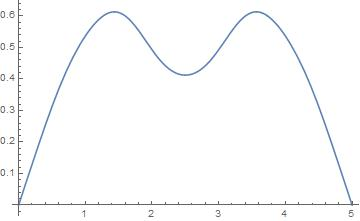
\includegraphics[width=5in]{out1}\\
  \caption{The plot of $\psi_1^{(1)}$}\label{out1}
\end{figure}

For the case $V_0=\frac{3\pi^2 \hbar^2}{ma^2}$, the plot of $\psi_1^{(1)}$ is shown in Figure \ref{out1}

\section{} %4

\subsection*{(a)}
When $\epsilon=0$, the Hamiltonian matrix becomes:

$$\mathbf{H}=V_0\left(
\begin{array}{ccc}
1 & 0 & 0 \\
0 & 1 & 0 \\
0 & 0 & 2
\end{array}
\right)$$

Suppose the eigenvalue is $E$ and the eigenvector is $|\psi^0\rangle$

Therefore, $\left(
\begin{array}{ccc}
V_0 & 0 & 0 \\
0 & V_0 & 0 \\
0 & 0 & 2V_0
\end{array}
\right) |\psi^0\rangle
=E|\psi^0\rangle$

$\therefore \left|
\begin{array}{ccc}
V_0-E & 0 & 0 \\
0 & V_0-E & 0 \\
0 & 0 & 2V_0-E
\end{array}
\right|=0$

$-E^3+4VE^2+5V^2E+2V^3=0$

$\therefore E=V_0 or 2V_0$

We let $|\psi^0\rangle =
\left(
\begin{array}{c}
a \\
b \\
c
\end{array}
\right)$

When $E=V_0$,

$\left(
\begin{array}{ccc}
V_0 & 0 & 0 \\
0 & V_0 & 0 \\
0 & 0 & 2V_0
\end{array}
\right)
\left(
\begin{array}{c}
a \\
b \\
c
\end{array}
\right)=
\left(
\begin{array}{c}
V_0a \\
V_0b \\
V_0c
\end{array}
\right)$

In this case, we can have two orthonormal eigenstates $\left(
\begin{array}{c}
1 \\
0 \\
0
\end{array}
\right)$ and $\left(
\begin{array}{c}
0 \\
1 \\
0
\end{array}
\right)$

When $E=2V_0$,

$\left(
\begin{array}{ccc}
V_0 & 0 & 0 \\
0 & V_0 & 0 \\
0 & 0 & 2V_0
\end{array}
\right)
\left(
\begin{array}{c}
a \\
b \\
c
\end{array}
\right)=
\left(
\begin{array}{c}
2V_0a \\
2V_0b \\
2V_0c
\end{array}
\right)$

In this case, we can have eigenstate $\left(
\begin{array}{c}
0 \\
0 \\
1
\end{array}
\right)$

\subsection*{(b)}
When the system is perturbed, we have

$$\mathbf{H}=V_0\left(
\begin{array}{ccc}
(1-\epsilon) & 0 & 0 \\
0 & 1 & \epsilon \\
0 & \epsilon & 2
\end{array}
\right)$$

Let the eigenvalue to be $E$ and the eigenvector to be $|\psi^1\rangle$

Then the eigenvalues are $E=(1-\epsilon)V_0$, $\frac{V_0}{2} (3-\sqrt{1+4\epsilon^2})$, $\frac{V_0}{2} (3+\sqrt{1+4\epsilon^2})$

Using power expansion, we can get $E=(1-\epsilon)V_0$, $\frac{V_0}{2} (3-1-2\epsilon^2)= V_0(1-\epsilon^2)$, $\frac{V_0}{2} (3+1+2\epsilon^2)=V_0(2+\epsilon^2)$

\subsection*{(c)}
From the question we can know that $H'=\epsilon V_0 \left(
\begin{array}{ccc}
-1 & 0 & 0 \\
0  & 0 & 1 \\
0  & 1 & 0
\end{array}
\right)
$

We let $|\psi_1^0\rangle=\left(
\begin{array}{c}
1 \\
0 \\
0
\end{array}
\right)$, $|\psi_2^0\rangle=\left(
\begin{array}{c}
0 \\
1 \\
0
\end{array}
\right)$ and $|\psi_3^0\rangle=\left(
\begin{array}{c}
0 \\
0 \\
1
\end{array}
\right)$

$\therefore E_1^1=\langle \psi_1^0 |H'| \psi_1^0 \rangle = \epsilon V_0\left(
\begin{array}{ccc}
1 & 0 & 0
\end{array}
\right)\left(
\begin{array}{ccc}
-1 & 0 & 0 \\
0  & 0 & 1 \\
0  & 1 & 0
\end{array}
\right)
\left(
\begin{array}{c}
1 \\
0 \\
0
\end{array}
\right)= -\epsilon V_0$

$E_2^1=\langle \psi_2^0 |H'| \psi_2^0 \rangle = \epsilon V_0\left(
\begin{array}{ccc}
0 & 1 & 0
\end{array}
\right)\left(
\begin{array}{ccc}
-1 & 0 & 0 \\
0  & 0 & 1 \\
0  & 1 & 0
\end{array}
\right)
\left(
\begin{array}{c}
0 \\
1 \\
0
\end{array}
\right)= 0$

$E_3^1=\langle \psi_3^0 |H'| \psi_3^0 \rangle = \epsilon V_0\left(
\begin{array}{ccc}
0 & 0 & 1
\end{array}
\right)\left(
\begin{array}{ccc}
-1 & 0 & 0 \\
0  & 0 & 1 \\
0  & 1 & 0
\end{array}
\right)
\left(
\begin{array}{c}
0 \\
0 \\
1
\end{array}
\right)= 0$

The equation for calculating the second order eigenvalues is $E_n^2=\sum_{m \ne n} \frac{|\langle \psi_m^0|H'| \psi_n^0 \rangle|^2}{E_n^0-E_m^0}$

Since $| \psi_1^0 \rangle$ and $| \psi_2^0 \rangle$ share the same eigenvalues $V_0$, the non-degenerate method only applies to $| \psi_3^0 \rangle$

Therefore, $E_3^2=\frac{|\langle \psi_1^0|H'| \psi_3^0 \rangle|^2}{E_3^0-E_1^0}+ \frac{|\langle \psi_2^0|H'| \psi_3^0 \rangle|^2}{E_3^0-E_2^0}= \frac{|\langle \psi_1^0|H'| \psi_3^0 \rangle|^2 + |\langle \psi_2^0|H'| \psi_3^0 \rangle|^2}{V_0}= \epsilon^2 V_0$

$E_3=E_3^0+E_3^1+E_3^2= 2V_0 + \epsilon^2 V_0 = V_0(2+\epsilon^2)$

This matches the answer in part (b)

\subsection*{(d)}
We let $\mathbf{W}=\left(
\begin{array}{ccc}
W_{11} & W_{12}  \\
W_{21} & W_{22}
\end{array}
\right)$, where $W_{ij}=\langle \psi_i^0 | H' | \psi_j^0 \rangle$

$\therefore W=\epsilon V_0 \left(
\begin{array}{cc}
-1 & 0\\
0  & 0
\end{array}
\right)$

The eigenvalues therefore are $E_1^1=-\epsilon V_0$ and $E_2^1=0$

$E_1=V_0-\epsilon V_0$ and $E_2=V_0$

This matches the results in (b) up to the first order of $\epsilon$

\section{} %5
\subsection*{(a)}
From the question we know that the perturbation matrix $H'=\left(
\begin{array}{cc}
H'_{11} & H'_{12}\\
H'_{21} & H'_{22}
\end{array}
\right)$, where $H'_{ij}= \langle \widetilde{\psi}_{2i}^{(0)} |H'| \widetilde{\psi}_{2j}^{(0)} \rangle$

We let $\widetilde{\psi}_{21}^{(0)}= \psi_{21}^{(0)}$ and $\widetilde{\psi}_{22}^{(0)}= \psi_{12}^{(0)}$

Plug in the values given in the question, we get

$H'_{11}=\int_{x=\frac{a}{2}}^a \int_{y=0}^{\frac{a}{2}} \widetilde{\psi}_{21}^{(0)}* \widetilde{\psi}_{21}^{(0)}* H'\ dy\ dx= \frac{\hbar ^2}{3 a^2 m}$

$H'_{12}=\int_{x=\frac{a}{2}}^a \int_{y=0}^{\frac{a}{2}} \widetilde{\psi}_{21}^{(0)}* \widetilde{\psi}_{22}^{(0)}* H'\ dy\ dx= -\frac{64 \hbar ^2}{225 a^2 m}$

$H'_{21}=\int_{x=\frac{a}{2}}^a \int_{y=0}^{\frac{a}{2}} \widetilde{\psi}_{22}^{(0)}* \widetilde{\psi}_{21}^{(0)}* H'\ dy\ dx=-\frac{64 \hbar ^2}{225 a^2 m}$

$H'_{22}=\int_{x=\frac{a}{2}}^a \int_{y=0}^{\frac{a}{2}} \widetilde{\psi}_{22}^{(0)}* \widetilde{\psi}_{22}^{(0)}* H'\ dy\ dx=\frac{\hbar ^2}{3 a^2 m}$

$$\therefore \boxed{ H'=\left(
\begin{array}{cc}
\frac{\hbar ^2}{3 a^2 m} & -\frac{64 \hbar ^2}{225 a^2 m} \\
-\frac{64 \hbar ^2}{225 a^2 m} & \frac{\hbar ^2}{3 a^2 m}
\end{array}
\right) }$$

\subsection*{(b)}
Suppose $\left(
\begin{array}{cc}
\frac{\hbar ^2}{3 a^2 m} & -\frac{64 \hbar ^2}{225 a^2 m} \\
-\frac{64 \hbar ^2}{225 a^2 m} & \frac{\hbar ^2}{3 a^2 m}
\end{array}
\right)\left(
\begin{array}{c}
c_1\\
c_2
\end{array}
\right)=E_2^{(1)}\left(
\begin{array}{c}
c_1\\
c_2
\end{array}
\right)$, where $\left(
\begin{array}{c}
c_1\\
c_2
\end{array}
\right)$ is the eigenstate and $E_2^{(1)}$ is the eigenvalue

We get that $E_2^{(1)}=\boxed{ \frac{139 \hbar ^2}{225 a^2 m}}$ or $\boxed{\frac{11 \hbar ^2}{225 a^2 m}}$

The corresponding eigenstates are $\left(
\begin{array}{c}
c_{11} \\
c_{12} \\
\end{array}
\right)=\boxed{ \left(
\begin{array}{c}
-1 \\
 1 \\
\end{array}
\right) }$ and $\left(
\begin{array}{c}
c_{21} \\
c_{22} \\
\end{array}
\right)=\boxed{ \left(
\begin{array}{c}
 1 \\
 1 \\
\end{array}
\right)}$

\subsection*{(c)}
According to part (b), when $E_2^{(1)}= \frac{139 \hbar ^2}{225 a^2 m}$

$|\phi_{21}^{(0)} \rangle= c_{11}|\widetilde{\psi}_{21}^{(0)}\rangle + c_{12}|\widetilde{\psi}_{22}^{(0)}\rangle = -\frac{2}{a} \sin(\frac{2\pi x}{a}) \sin(\frac{\pi y}{a})+ \frac{2}{a}\sin(\frac{\pi x}{a}) \sin(\frac{2\pi y}{a})$

\begin{figure}
  \centering
  % Requires \usepackage{graphicx}
  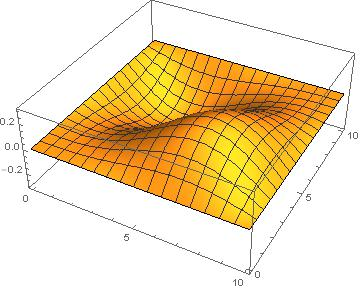
\includegraphics[width=5in]{out2}\\
  \caption{The plot of $|\phi_{21}^{(0)} \rangle$} \label{out2}
\end{figure}

The Plot of $|\phi_{21}^{(0)} \rangle$ is shown in Figure \ref{out2}

when $E_2^{(1)}= \frac{11 \hbar ^2}{225 a^2 m}$

\begin{figure}
  \centering
  % Requires \usepackage{graphicx}
  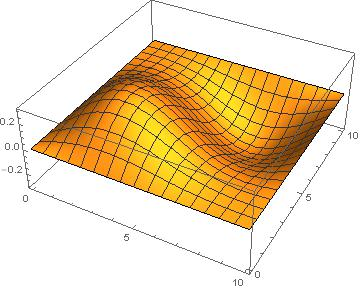
\includegraphics[width=5in]{out3}\\
  \caption{The plot of $|\phi_{22}^{(0)} \rangle$}\label{out3}
\end{figure}

$|\phi_{22}^{(0)} \rangle= c_{21}|\widetilde{\psi}_{21}^{(0)}\rangle + c_{22}|\widetilde{\psi}_{22}^{(0)}\rangle = \frac{2}{a} \sin(\frac{2\pi x}{a}) \sin(\frac{\pi y}{a})+ \frac{2}{a}\sin(\frac{\pi x}{a}) \sin(\frac{2\pi y}{a})$

The Plot of $|\phi_{22}^{(0)} \rangle$ is shown in Figure \ref{out3}

According to Figure \ref{out2} and Figure \ref{out3}, we can see that $|\phi_{21}^{(0)} \rangle$ has higher amplitude than $|\phi_{22}^{(0)} \rangle$ in the perturbation area. Therefore the energy with eigenstate $|\phi_{21}^{(0)} \rangle$ is higher

\end{spacing}
\end{document} 